% Section VI: Results and discussion (target 1.50 pages with Table IV and Fig. 3).
% Sources: data/eval/eval_sheet.csv (operator-confirmed judgments), data/policy/run_real_20261031_*.csv/.json/.mp4,
% docs/experiments.md (evaluation row), docs/decisions.md t3-g addendum 3.
\section{Results and Discussion}
\label{sec:results}

\subsection{Packing Performance}
\label{sec:performance}
Of the 20 trials, 12 were complete successes (60\%; Wilson 95\% interval
39--78\%), and 11 of these also kept the demonstrated order.
Table~\ref{tab:results} breaks the outcome down by item and by layout. Of the
60 items, 49 were placed correctly. No item was released into a wrong
compartment: every item that reached the place stage ended in its assigned
container, except one RITZ that came to rest on the rim of the small hole.
The losses occur earlier. The Oreo was lost mainly during transport (16 of 19
grasped Oreos reached a container) and the RITZ at the grasp (15 of 19
attempted). The carrot was grasped in 19 of 20 trials and then always placed;
the exception is the trial with an intervention.

The layouts differ more than the items. L1 and L4 succeeded in all four
trials with every item placed, whereas L2 and L3 succeeded once each. The
successful trials took a median of 54.1~s from the start key to the last
release (mean 56.9~s, range 40.4--82.6~s). The three-item demonstrations lasted
58.8~s on average under a longer measure (start to end of recording), so the
policy packs at roughly the pace of teleoperation rather than faster.
Fig.~\ref{fig:sequence} shows the fastest trial.

\begin{table}[t]
\caption{Evaluation Results (20 Trials)}
\label{tab:results}
\centering
\footnotesize
\setlength{\tabcolsep}{3.5pt}
\begin{tabular}{@{}lccccc@{}}
\toprule
\multicolumn{6}{@{}l}{(a) Stage rates per item, conditional on reaching the stage}\\
Item & Grasp & Transport & Place & Correct & Correct / 20\\
\midrule
Carrot & 19/20 & 19/19 & 19/19 & 19/19 & 19\\
Oreo & 19/20 & 16/19 & 16/16 & 16/16 & 16\\
RITZ & 15/19 & 15/15 & 14/15 & 14/14 & 14\\
\midrule
\multicolumn{6}{@{}l}{(b) Per layout}\\
Layout & Complete & \multicolumn{2}{c}{Correct items} & \multicolumn{2}{l}{Main failure causes}\\
\midrule
L1 & 4/4 & \multicolumn{2}{c}{12/12} & \multicolumn{2}{l}{--}\\
L2 & 1/4 & \multicolumn{2}{c}{9/12} & \multicolumn{2}{l}{RITZ not approached (2), rim (1)}\\
L3 & 1/4 & \multicolumn{2}{c}{6/12} & \multicolumn{2}{l}{Oreo displaced (3)}\\
L4 & 4/4 & \multicolumn{2}{c}{12/12} & \multicolumn{2}{l}{--}\\
L5 & 2/4 & \multicolumn{2}{c}{10/12} & \multicolumn{2}{l}{intervention (1), slip (1)}\\
\midrule
All & 12/20 & \multicolumn{2}{c}{49/60} & \multicolumn{2}{l}{}\\
\bottomrule
\end{tabular}
% One RITZ was not attempted (trial 20). Intervention: trial 5 (carrot re-placed by hand).
\end{table}

\begin{figure}[t]
\centering
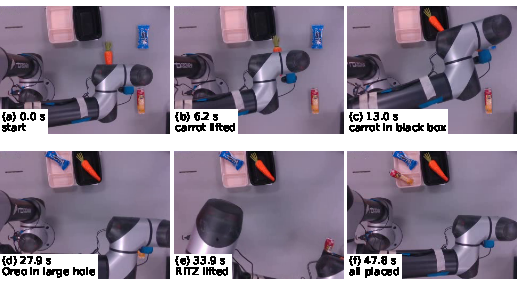
\includegraphics[width=\columnwidth]{figures/fig3_sequence.pdf}
\caption{A complete autonomous packing sequence (trial 18, layout L1), seen by
the front camera. Times are from the start key; the last release was at 40.4~s.}
\label{fig:sequence}
\end{figure}
% Made by paper/figures/make_fig3.py from data/policy/run_real_20261031_070212 (releases 9.4, 23.2, 40.4 s
% after the start key; resting items shown halfway between a release and the next close).

\subsection{Grasping and Recovery}
\label{sec:grasping}
Of the 59 attempted items, 29 were grasped at the first close. Grasping
again after a miss was common: after an empty close, the policy reopened,
moved above the item, and closed again, as shown in the recovery
demonstrations. In total, 24 of the 30 items with a miss were eventually
grasped (carrot 11/12, Oreo 7/8, RITZ 6/10). In the 12 successful trials, the
gripper closed 65 times for 36 items, 1.8 times per item. Over all trials,
only 54 of 181 closes lifted an item, but 94 of the closes came from the four
trials in which the policy stalled (Section~\ref{sec:failures}). No policy
trained without recovery demonstrations was tested under the same protocol, so
these numbers describe the evaluated policy and do not measure what the
recovery episodes contributed.

\subsection{Failure Analysis and Operational Behavior}
\label{sec:failures}
Eight trials failed. \emph{Items displaced from demonstrated states} caused
three, all in L3, where the Oreo lies nearest the robot. The fingers closed
on its edge; in two trials the Oreo was lifted and fell on the way, beside
the black box, and in the third it was pushed there without being grasped.
The policy then closed repeatedly at a fixed empty spot, every 5--6~s, until
the time limit, and neither the Oreo nor the RITZ was grasped. An item lying
next to a container never appears in the training data: episodes with a
dropped item were discarded (Section~\ref{sec:protocol}), and the recovery
episodes only show re-grasps near the item.
\emph{A far item not approached} caused two failures in L2. After placing
the carrot and the Oreo, the policy moved to an empty area about 25~cm from
the RITZ, which lay at the front edge of the item region, and stalled. The same
layout succeeded once, and in its fourth trial the RITZ ended on the rim of
the small hole. The remaining two failures occurred in L5. In one, the Oreo
was taken before the carrot, held near the fingertips, and slipped out on the
way. In the other, the gripper pushed the carrot and turned it to an
orientation that the fingers could not close across. The operator re-placed
it, so the trial counts as failed. Because the tool orientation follows a
fixed rule (Section~\ref{sec:interface}) rather than being learned, a rotated
item cannot be grasped.

The packing order was broken three times, all in L5: after missing or
displacing the carrot, the policy carried the Oreo first. The RITZ was never
carried before the Oreo. In L4, where the RITZ lies nearest, the first reach
went to the RITZ in all four trials; after missing it, the policy turned to
the carrot and completed all four trials in order. The order was therefore
learned, but proximity could take over when the next item in the order was
not grasped.

Execution was stable throughout. Over 54{,}167 predictions (28.2 per second),
inference took 23.6~ms at the median and 49.1~ms at the 95th percentile. The
servo interval had a median of 20.0~ms and a maximum of 40.3~ms, and 30 of
95{,}913 cycles were late. No hold was triggered, no robot state was stale,
and every run was closed with the operator's key, five of them after the time
limit; none ended with a controller stop.

\subsection{Application Scope and Limitations}
\label{sec:limitations}
The evidence comes from one policy, one training run, and one session; 20
trials leave a wide confidence interval. The layouts lie inside the
demonstrated item region, the items keep their demonstrated orientations, and
the containers, lighting, and model foods are fixed. Within this scope,
placement was reliable, and the limiting factors were grasping and continuing
from states the demonstrations do not cover. Demonstrations that pick up items
lying beside the containers, wider coverage near the robot and at the far edge
of the item region, and a perceived rather than fixed tool orientation are the
direct next steps. The task-space interface connects the dissimilar leader and
follower; it does not establish transfer to another follower. The study makes
no claim about real food, unseen objects, industrial readiness, or safety.
